ONAR MMSoft is a company that located at Jouy-en-Josas in France.
It's part of the group ONAR MMCall, which specializes in the distribution
of pagers.
It offers software solutions majorly for workflow management, which
are mostly based on making use of pagers.

\begin{figure}[!htpb]
    \centering
    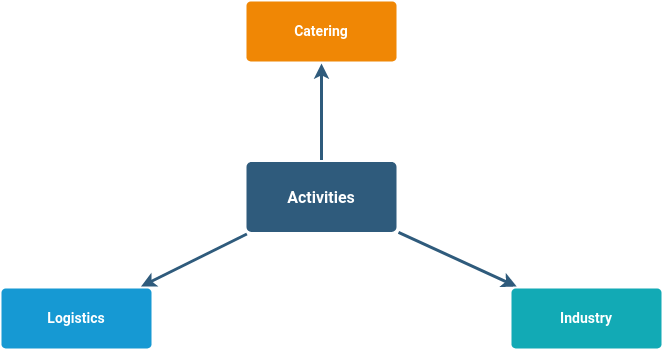
\includegraphics[width=0.8\textwidth]{images/core_activities.png}
    \caption{\footnotesize{Organization core activities}}
    \label{fig:core_activities}
\end{figure}

As of today and as shown in \ref{fig:core_activities}, the company has
interest in several fields of activities:
\begin{itemize}
    \item Catering
    \item Logistics
    \item Manufacturing
\end{itemize}

Mainly handling problems related to management workflows for those fields,
lately turning all it focus into the field of logistics.

Some of the solutions that the company has developed and is maintaining are:
\begin{itemize}
    \item Ultim R which is composed of an App to order lunch, an IT tool to manage kitchen
        operations from dishes preparation to order management and a module for plates
        delivery which was for the client RATP.

    \item A solution developed for Autoneum which was focused on reducing the time
        spent with production workstations on factories. Offering also statistics
        and a recommender system to help reduct lead-time, alert function to 
        inform of accident cases.

    \item Easy Truck In a solution for the management of trucks, which is a winner of an
        ID Logistics interval innovation contest, it provides easy access to the logistics
        platform, support operational teams, eases check-in and access controls and
        offering access to visual management tools.
\end{itemize}

\begin{figure}[!htpb]
    \centering
    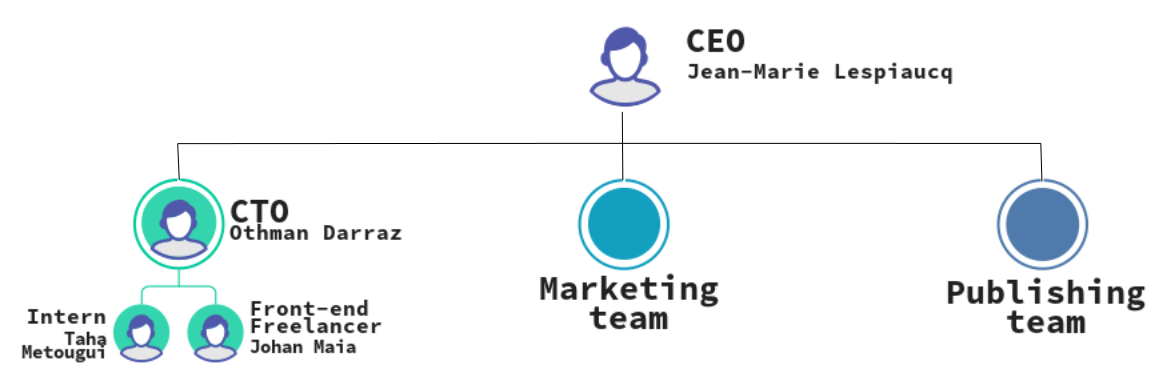
\includegraphics[width=\textwidth]{images/Hierarchy.png}
    \caption{\footnotesize{Organization chart of the company}}
    \label{fig:core_activities_2}
\end{figure}

The organisation unit, I've integrated, is composed of three members,
the CTO "Othman Darraz" who's in charge of managing the project, reviewing new modules
and PR requests, a freelancer "Johan Maia" who's in charge of everything that's front-end
from web application to phone application, and me joining them as the third member of the
team to partake in the backend and infrastructure mainly refactoring, security and
improving the infrastructure from virtualisation to deployment.

